\documentclass[]{book}
\usepackage{lmodern}
\usepackage{amssymb,amsmath}
\usepackage{ifxetex,ifluatex}
\usepackage{fixltx2e} % provides \textsubscript
\ifnum 0\ifxetex 1\fi\ifluatex 1\fi=0 % if pdftex
  \usepackage[T1]{fontenc}
  \usepackage[utf8]{inputenc}
\else % if luatex or xelatex
  \ifxetex
    \usepackage{mathspec}
  \else
    \usepackage{fontspec}
  \fi
  \defaultfontfeatures{Ligatures=TeX,Scale=MatchLowercase}
\fi
% use upquote if available, for straight quotes in verbatim environments
\IfFileExists{upquote.sty}{\usepackage{upquote}}{}
% use microtype if available
\IfFileExists{microtype.sty}{%
\usepackage[]{microtype}
\UseMicrotypeSet[protrusion]{basicmath} % disable protrusion for tt fonts
}{}
\PassOptionsToPackage{hyphens}{url} % url is loaded by hyperref
\usepackage[unicode=true]{hyperref}
\hypersetup{
            pdftitle={Data Network Dashboards},
            pdfauthor={This document is currently under construction},
            pdfborder={0 0 0},
            breaklinks=true}
\urlstyle{same}  % don't use monospace font for urls
\usepackage{natbib}
\bibliographystyle{apalike}
\usepackage{color}
\usepackage{fancyvrb}
\newcommand{\VerbBar}{|}
\newcommand{\VERB}{\Verb[commandchars=\\\{\}]}
\DefineVerbatimEnvironment{Highlighting}{Verbatim}{commandchars=\\\{\}}
% Add ',fontsize=\small' for more characters per line
\usepackage{framed}
\definecolor{shadecolor}{RGB}{248,248,248}
\newenvironment{Shaded}{\begin{snugshade}}{\end{snugshade}}
\newcommand{\KeywordTok}[1]{\textcolor[rgb]{0.13,0.29,0.53}{\textbf{#1}}}
\newcommand{\DataTypeTok}[1]{\textcolor[rgb]{0.13,0.29,0.53}{#1}}
\newcommand{\DecValTok}[1]{\textcolor[rgb]{0.00,0.00,0.81}{#1}}
\newcommand{\BaseNTok}[1]{\textcolor[rgb]{0.00,0.00,0.81}{#1}}
\newcommand{\FloatTok}[1]{\textcolor[rgb]{0.00,0.00,0.81}{#1}}
\newcommand{\ConstantTok}[1]{\textcolor[rgb]{0.00,0.00,0.00}{#1}}
\newcommand{\CharTok}[1]{\textcolor[rgb]{0.31,0.60,0.02}{#1}}
\newcommand{\SpecialCharTok}[1]{\textcolor[rgb]{0.00,0.00,0.00}{#1}}
\newcommand{\StringTok}[1]{\textcolor[rgb]{0.31,0.60,0.02}{#1}}
\newcommand{\VerbatimStringTok}[1]{\textcolor[rgb]{0.31,0.60,0.02}{#1}}
\newcommand{\SpecialStringTok}[1]{\textcolor[rgb]{0.31,0.60,0.02}{#1}}
\newcommand{\ImportTok}[1]{#1}
\newcommand{\CommentTok}[1]{\textcolor[rgb]{0.56,0.35,0.01}{\textit{#1}}}
\newcommand{\DocumentationTok}[1]{\textcolor[rgb]{0.56,0.35,0.01}{\textbf{\textit{#1}}}}
\newcommand{\AnnotationTok}[1]{\textcolor[rgb]{0.56,0.35,0.01}{\textbf{\textit{#1}}}}
\newcommand{\CommentVarTok}[1]{\textcolor[rgb]{0.56,0.35,0.01}{\textbf{\textit{#1}}}}
\newcommand{\OtherTok}[1]{\textcolor[rgb]{0.56,0.35,0.01}{#1}}
\newcommand{\FunctionTok}[1]{\textcolor[rgb]{0.00,0.00,0.00}{#1}}
\newcommand{\VariableTok}[1]{\textcolor[rgb]{0.00,0.00,0.00}{#1}}
\newcommand{\ControlFlowTok}[1]{\textcolor[rgb]{0.13,0.29,0.53}{\textbf{#1}}}
\newcommand{\OperatorTok}[1]{\textcolor[rgb]{0.81,0.36,0.00}{\textbf{#1}}}
\newcommand{\BuiltInTok}[1]{#1}
\newcommand{\ExtensionTok}[1]{#1}
\newcommand{\PreprocessorTok}[1]{\textcolor[rgb]{0.56,0.35,0.01}{\textit{#1}}}
\newcommand{\AttributeTok}[1]{\textcolor[rgb]{0.77,0.63,0.00}{#1}}
\newcommand{\RegionMarkerTok}[1]{#1}
\newcommand{\InformationTok}[1]{\textcolor[rgb]{0.56,0.35,0.01}{\textbf{\textit{#1}}}}
\newcommand{\WarningTok}[1]{\textcolor[rgb]{0.56,0.35,0.01}{\textbf{\textit{#1}}}}
\newcommand{\AlertTok}[1]{\textcolor[rgb]{0.94,0.16,0.16}{#1}}
\newcommand{\ErrorTok}[1]{\textcolor[rgb]{0.64,0.00,0.00}{\textbf{#1}}}
\newcommand{\NormalTok}[1]{#1}
\usepackage{longtable,booktabs}
% Fix footnotes in tables (requires footnote package)
\IfFileExists{footnote.sty}{\usepackage{footnote}\makesavenoteenv{long table}}{}
\usepackage{graphicx,grffile}
\makeatletter
\def\maxwidth{\ifdim\Gin@nat@width>\linewidth\linewidth\else\Gin@nat@width\fi}
\def\maxheight{\ifdim\Gin@nat@height>\textheight\textheight\else\Gin@nat@height\fi}
\makeatother
% Scale images if necessary, so that they will not overflow the page
% margins by default, and it is still possible to overwrite the defaults
% using explicit options in \includegraphics[width, height, ...]{}
\setkeys{Gin}{width=\maxwidth,height=\maxheight,keepaspectratio}
\IfFileExists{parskip.sty}{%
\usepackage{parskip}
}{% else
\setlength{\parindent}{0pt}
\setlength{\parskip}{6pt plus 2pt minus 1pt}
}
\setlength{\emergencystretch}{3em}  % prevent overfull lines
\providecommand{\tightlist}{%
  \setlength{\itemsep}{0pt}\setlength{\parskip}{0pt}}
\setcounter{secnumdepth}{5}
% Redefines (sub)paragraphs to behave more like sections
\ifx\paragraph\undefined\else
\let\oldparagraph\paragraph
\renewcommand{\paragraph}[1]{\oldparagraph{#1}\mbox{}}
\fi
\ifx\subparagraph\undefined\else
\let\oldsubparagraph\subparagraph
\renewcommand{\subparagraph}[1]{\oldsubparagraph{#1}\mbox{}}
\fi

% set default figure placement to htbp
\makeatletter
\def\fps@figure{htbp}
\makeatother

\usepackage{booktabs}
\usepackage{amsthm}
\makeatletter
\def\thm@space@setup{%
  \thm@preskip=8pt plus 2pt minus 4pt
  \thm@postskip=\thm@preskip
}
\makeatother

\title{Data Network Dashboards}
\author{This document is currently under construction}
\date{2020-03-03}

\begin{document}
\maketitle

{
\setcounter{tocdepth}{1}
\tableofcontents
}
\chapter*{Preface}\label{preface}
\addcontentsline{toc}{chapter}{Preface}

\textbf{This document is currently under construction}

Automated Characterization of Health Information at Large-scale
Longitudinal Evidence Systems (ACHILLES) is a profiling tool developed
by the OHDSI community to provide descriptive statistics of databases
standardized to the OMOP Common Data Model. These characteristics are
presented graphically in the ATLAS tool. However, this solution does not
allow for database comparison across the data network. The proposed
solution aggregates ACHILLES results files from databases in the network
and displays the descriptive statistics through graphical dashboards.
The tool is helpful to gain insight in the growth of the data network
and is useful for the selection of databases for specific research
questions. In the software demonstration we show a first version of this
tool that will be further developed in EHDEN in close collaboration with
all our stakeholders, including OHDSI.

\section*{Goals}\label{goals}
\addcontentsline{toc}{section}{Goals}

This manual aims to document the procedures to install and configure the
chasrts and dashboards choosen to compare the OHDSI databases.

\ldots{}.

\section*{Contributors}\label{contributors}
\addcontentsline{toc}{section}{Contributors}

To develop this tool, EHDEN organized a hack-a-thon (Aveiro, December
2-3, 2019), where we defined and implemented a series of charts and
dashboards containing the most relevant information about the databases.
The team involved in this task were composed by the following members:

\begin{itemize}
\tightlist
\item
  João Rafael Almeida\textsuperscript{1}
\item
  André Pedrosa\textsuperscript{1}
\item
  Peter R. Rijnbeek\textsuperscript{2}
\item
  Marcel de Wilde\textsuperscript{2}
\item
  Michel Van Speybroeck\textsuperscript{3}
\item
  Maxim Moinat\textsuperscript{4}
\item
  Pedro Freire\textsuperscript{1}
\item
  Alina Trifan\textsuperscript{1}
\item
  Sérgio Matos\textsuperscript{1}
\item
  José Luís Oliveira\textsuperscript{1}
\end{itemize}

1 - Institute of Electronics and Informatics Engineering of Aveiro,
Department of Electronics and Telecommunication, University of Aveiro,
Aveiro, Portugal

2 - Erasmus MC, Rotterdam, Netherlands

3 - Janssen Pharmaceutica NV, Beerse, Belgium

4 - The Hyve, Utrecht, Netherlands

\section*{License}\label{license}
\addcontentsline{toc}{section}{License}

The system is open-source under the license \ldots{}.

The book is written in \href{https://rmarkdown.rstudio.com}{RMarkdown}
using the \href{https://bookdown.org}{bookdown} package.

\section*{Acknowledges}\label{acknowledges}
\addcontentsline{toc}{section}{Acknowledges}

This work has been conducted in the context of EHDEN, a project that
receives funding from the European Union's Horizon 2020 and EFPIA
through IMI2 Joint Undertaking initiative, under grant agreement No
806968.

\chapter{Introduction}\label{introduction}

The OHDSI research network has been growing steadily which results in an
increasing number of healthcare databases standardized to the OMOP CDM
format. The OHDSI community created the ACHILLES tool (Automated
Characterization of Health Information at Large-scale Longitudinal
Exploration System) to characterize those databases. The results are
available to the data custodian in their local ATLAS tool and helps them
to gain insights in their data and helps in assessing the feasibility of
a particular research questions.

ACHILLES was designed to extract the metadata from a single database,
which by itself does not allow the comparison with the remaining
databases in the network. However, we believe there is even more value
in sharing this information with others to enable network research in a
Data Network Dashboard.

\section{Data Network Dashboard}\label{data-network-dashboard}

The European Health Data and Evidence Network (EHDEN) project therefore
designed a Data Network Dashboard tool, a web application to aggregate
information from distributed OMOP CDM databases. It uses the ACHILLES
results files to construct graphical dashboards and enables database
comparison (Figure \ref{fig:cdmBI}). The tool is built on Apache
Superset, which is an open-source enterprise-ready business intelligence
web application that can provide powerful and fully customizable
graphical representations of data. Achilles results can be uploaded
through the EHDEN Database Catalogue using the dashboards plugin but can
also be directly uploaded in the tool. Figure 1. Example of a dashboards
tool presenting age and gender distributions (simulated data).

\begin{figure}
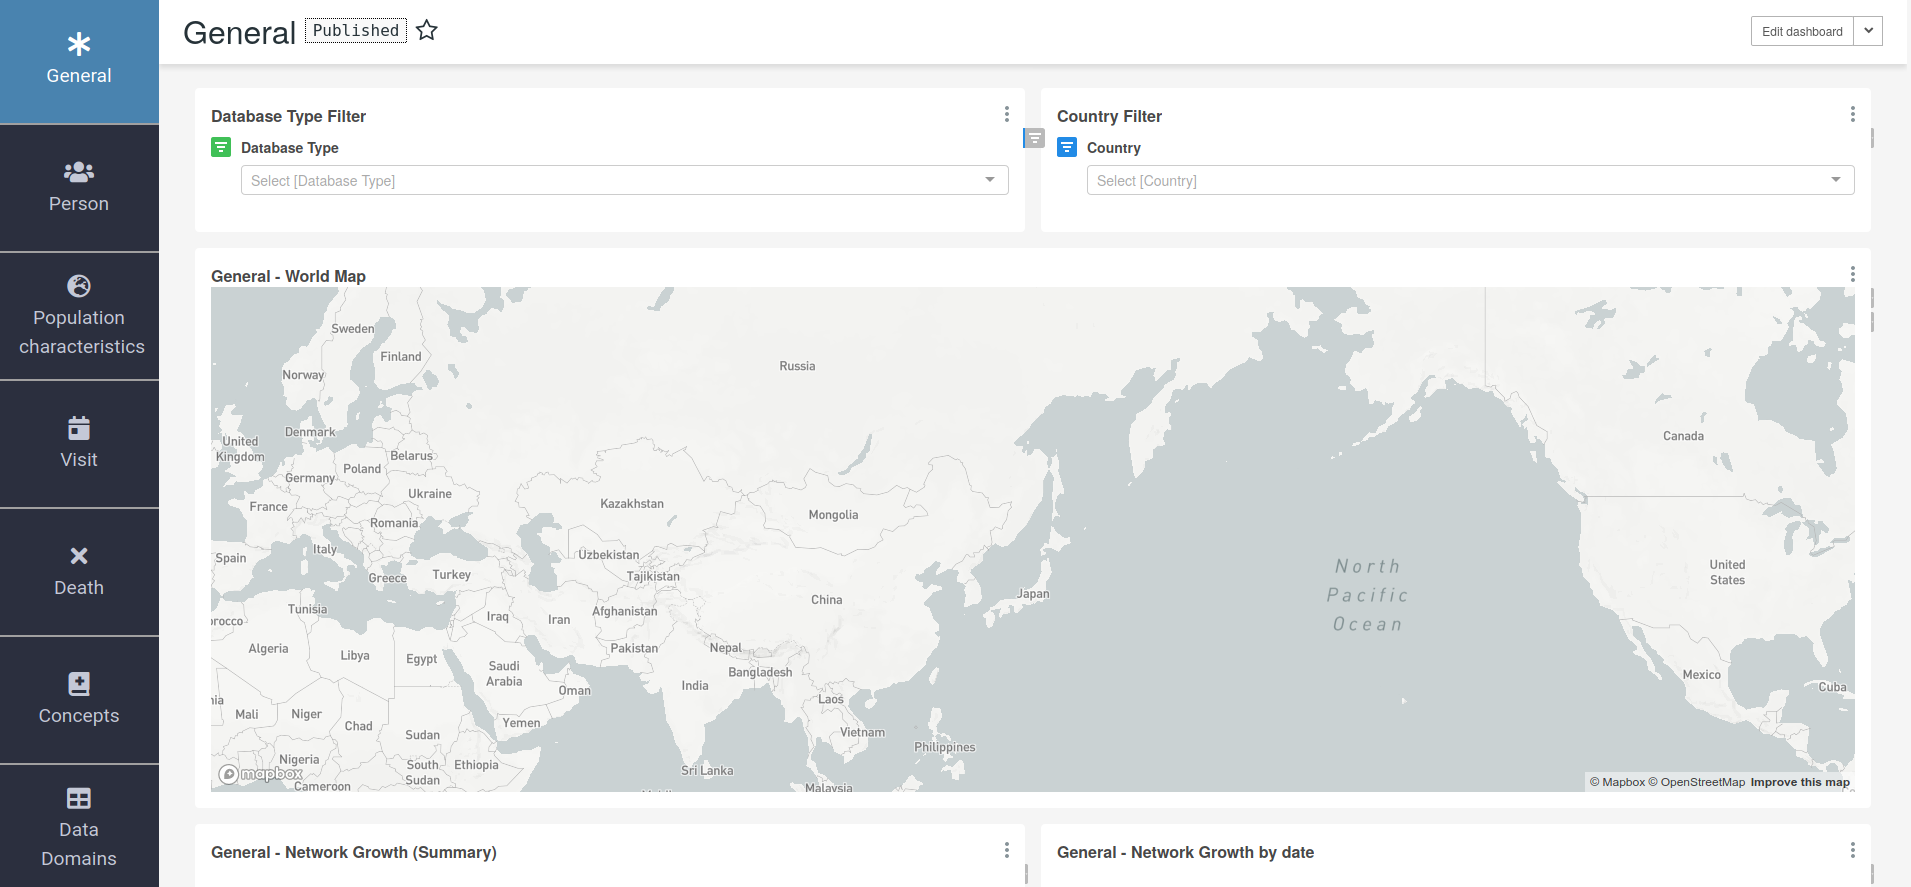
\includegraphics[width=1\linewidth]{images/cdmBI} \caption{Example of a dashboards tool presenting the databases available in the network (simulated data)}\label{fig:cdmBI}
\end{figure}

In this tools, we defined and implemented a series of charts and
dashboards containing the most relevant information about the databases,
such as:

\begin{itemize}
\tightlist
\item
  \textbf{General}: dashboards that shows the databases types per
  country, the distribution of data source types, the growth of the
  Network including the number of database and the number of patients in
  the databases over time;
\item
  \textbf{Person}: representing the number of patients per country, age
  distribution at first observation, year of birth distribution and
  normalized gender distribution;
\item
  \textbf{Population characteristics}: dashboard with the cumulative
  patient time, persons with continuous observation per month, and the
  start and end dates of those periods;
\item
  \textbf{Visit}: chart to compare the number and type of visit
  occurrence records;
\item
  \textbf{Death}: information about the number of death records by
  month, and the patient age at time of death;
\item
  \textbf{Concepts}: bubble chart which shows the number of patients and
  records per concept over the databases;
\item
  \textbf{Data domains}: heat map visualization of the major data
  domains in each database.
\end{itemize}

\chapter{Installation}\label{installation}

Make sure that you have docker and docker-compose installed in your
machine. Then, please follow these steps:

\begin{itemize}
\item
  Please enter in the `'docker'' directory and create your \texttt{.env}
  file here, using \texttt{.env-example} as reference. For local
  installation, you can just copy the \texttt{.env-example} content to a
  new file. Note: In case of port errors in the next steps, the problem
  could be related to a port already in use by your system that you
  defined here and it is busy, chose other.
\item
  Tip the following commands in the command line:

  \begin{enumerate}
  \def\labelenumi{\arabic{enumi}.}
  \item
    Clone the Apache Superset repository:

\begin{verbatim}
git clone https://github.com/apache/incubator-superset
 ../superset
cp ../superset/contrib/docker/superset_config.py ../superset
\end{verbatim}
  \item
    Init the Apache Superset (This creates a user, so it is necessary to
    interact with the console):

\begin{verbatim}
docker-compose run --rm superset ./docker-init.sh
\end{verbatim}
  \item
    Init the Dashboard Layout (This creates a user, so it is necessary
    to interact with the console):

\begin{verbatim}
docker-compose run --rm dashboard_viewer ./docker-init.sh
\end{verbatim}
  \item
    Finally, bring up the containers

\begin{verbatim}
docker-compose up -d
\end{verbatim}
  \end{enumerate}
\end{itemize}

To check if everything is ok, please wait 2 minutes and tip
\texttt{docker\ ps} and the following containers need to be running:

\begin{verbatim}
... 0.0.0.0:8088->8088/tcp   dashboard_viewer_superset_1
... 0.0.0.0:8000->8000/tcp   dashboard_viewer_dashboard_viewer_1
... 0.0.0.0:6379->6379/tcp   dashboard_viewer_redis_1
... 5432/tcp                 dashboard_viewer_postgres_1
\end{verbatim}

Now, you have a clean setup running in your machine. To try the
application using synthetic data, please continue to follow the steps in
the `'Demo'' section.

\section{Insert Concepts}\label{insert-concepts}

The concepts table are not in the repository due to its dimension.
Therefore, to insert this table in the installation, you should perform
the following steps:

\begin{enumerate}
\def\labelenumi{\arabic{enumi}.}
\item
  Download concept.csv file from here (todo)
\item
  Copy the file to the /tmp directory inside of the postgres container

\begin{Shaded}
\begin{Highlighting}[]
\ExtensionTok{docker}\NormalTok{ cp concept.csv dashboard_viewer_postgres_1:/tmp/}
\end{Highlighting}
\end{Shaded}
\item
  Enter in the dashboard\_viewer\_postgres\_1 container:

\begin{Shaded}
\begin{Highlighting}[]
\ExtensionTok{docker}\NormalTok{ exec -it dashboard_viewer_postgres_1 bash}
\end{Highlighting}
\end{Shaded}
\item
  Enter in the achilles database:

\begin{verbatim}
psql achilles
\end{verbatim}
\item
  Create the table in the database using this command:

\begin{Shaded}
\begin{Highlighting}[]
    \KeywordTok{CREATE} \KeywordTok{TABLE}\NormalTok{ concept (}
\NormalTok{      concept_id         }\DataTypeTok{INTEGER}        \KeywordTok{NOT} \KeywordTok{NULL}\NormalTok{,}
\NormalTok{      concept_name       }\DataTypeTok{VARCHAR}\NormalTok{(}\DecValTok{255}\NormalTok{)   }\KeywordTok{NOT} \KeywordTok{NULL}\NormalTok{,}
\NormalTok{      domain_id          }\DataTypeTok{VARCHAR}\NormalTok{(}\DecValTok{20}\NormalTok{)    }\KeywordTok{NOT} \KeywordTok{NULL}\NormalTok{,}
\NormalTok{      vocabulary_id      }\DataTypeTok{VARCHAR}\NormalTok{(}\DecValTok{20}\NormalTok{)    }\KeywordTok{NOT} \KeywordTok{NULL}\NormalTok{,}
\NormalTok{      concept_class_id   }\DataTypeTok{VARCHAR}\NormalTok{(}\DecValTok{20}\NormalTok{)    }\KeywordTok{NOT} \KeywordTok{NULL}\NormalTok{,}
\NormalTok{      standard_concept   }\DataTypeTok{VARCHAR}\NormalTok{(}\DecValTok{1}\NormalTok{)     }\KeywordTok{NULL}\NormalTok{,}
\NormalTok{      concept_code       }\DataTypeTok{VARCHAR}\NormalTok{(}\DecValTok{50}\NormalTok{)    }\KeywordTok{NOT} \KeywordTok{NULL}\NormalTok{,}
\NormalTok{      valid_start_date   }\DataTypeTok{DATE}           \KeywordTok{NOT} \KeywordTok{NULL}\NormalTok{,}
\NormalTok{      valid_end_date     }\DataTypeTok{DATE}           \KeywordTok{NOT} \KeywordTok{NULL}\NormalTok{,}
\NormalTok{      invalid_reason     }\DataTypeTok{VARCHAR}\NormalTok{(}\DecValTok{1}\NormalTok{)     }\KeywordTok{NULL}
\NormalTok{    );}
\end{Highlighting}
\end{Shaded}
\item
  Copy the CSV file content to the table (this could take a while):

\begin{Shaded}
\begin{Highlighting}[]
\KeywordTok{COPY}\NormalTok{ public.concept }\KeywordTok{from} \StringTok{'/tmp/concept.csv'} \KeywordTok{WITH}\NormalTok{ DELIMITER }\StringTok{','}
\NormalTok{    CSV }\KeywordTok{HEADER}\NormalTok{;}
\end{Highlighting}
\end{Shaded}
\item
  Alter table ownership:

\begin{Shaded}
\begin{Highlighting}[]
\CommentTok{-- <user> : defined in the .env file}
\KeywordTok{ALTER} \KeywordTok{TABLE}\NormalTok{ public.concept OWNER }\KeywordTok{TO}\NormalTok{ <user>;}
\end{Highlighting}
\end{Shaded}
\item
  Create index in table:

\begin{Shaded}
\begin{Highlighting}[]
\KeywordTok{CREATE} \KeywordTok{INDEX}\NormalTok{ achilles_results_analysis_id_index }\KeywordTok{ON} 
\NormalTok{    achilles_results (analysis_id);}
\KeywordTok{CREATE} \KeywordTok{INDEX}\NormalTok{ achilles_results_source_index }\KeywordTok{ON}\NormalTok{ achilles_results }
\NormalTok{    (data_source_id);}
\KeywordTok{CREATE} \KeywordTok{INDEX}\NormalTok{ concept_concept_id_index }\KeywordTok{ON}\NormalTok{ concept (concept_id);}
\KeywordTok{CREATE} \KeywordTok{INDEX}\NormalTok{ concept_concept_name_index }\KeywordTok{ON}\NormalTok{ concept }
\NormalTok{    (concept_name);}
\end{Highlighting}
\end{Shaded}
\end{enumerate}

\section{Import dashboards}\label{import-dashboards}

TO DO

\section{Dummy data}\label{dummy-data}

TO DO

\chapter{General}\label{general}

Discuss the goal of this dashboard\ldots{} TO DO

\section{Database Type Filter}\label{database-type-filter}

This filter which is a type of chart in Superset was designed to be used
in the dashboard aiming the filtering of the data based on the field
`'database\_type'`from the table'`data\_source'`. It is important to
give the alias'`Type'' to this field in the select operations because
Superset does not recognize as the same field otherwise. \#\#\# SQL
query

\begin{Shaded}
\begin{Highlighting}[]
\CommentTok{--  Country and database type filters}
\KeywordTok{SELECT}\NormalTok{ source.name, }
\NormalTok{       country.country }\KeywordTok{AS}\NormalTok{ Country, }
\NormalTok{       database_type }\KeywordTok{AS} \KeywordTok{Type}\NormalTok{,}
\NormalTok{       source.slug}
\KeywordTok{FROM}\NormalTok{ public.data_source }\KeywordTok{AS} \KeywordTok{source} \KeywordTok{INNER} \KeywordTok{JOIN}\NormalTok{ public.country }
  \KeywordTok{AS}\NormalTok{ country }\KeywordTok{ON}\NormalTok{ source.country_id=country.id;}
\end{Highlighting}
\end{Shaded}

\subsection{Chart settings}\label{chart-settings}

The main characteristics of this chart are presented in Figure
\ref{fig:databaseTypeFilter}, being the following:

\begin{itemize}
\tightlist
\item
  todo
\end{itemize}

\begin{figure}
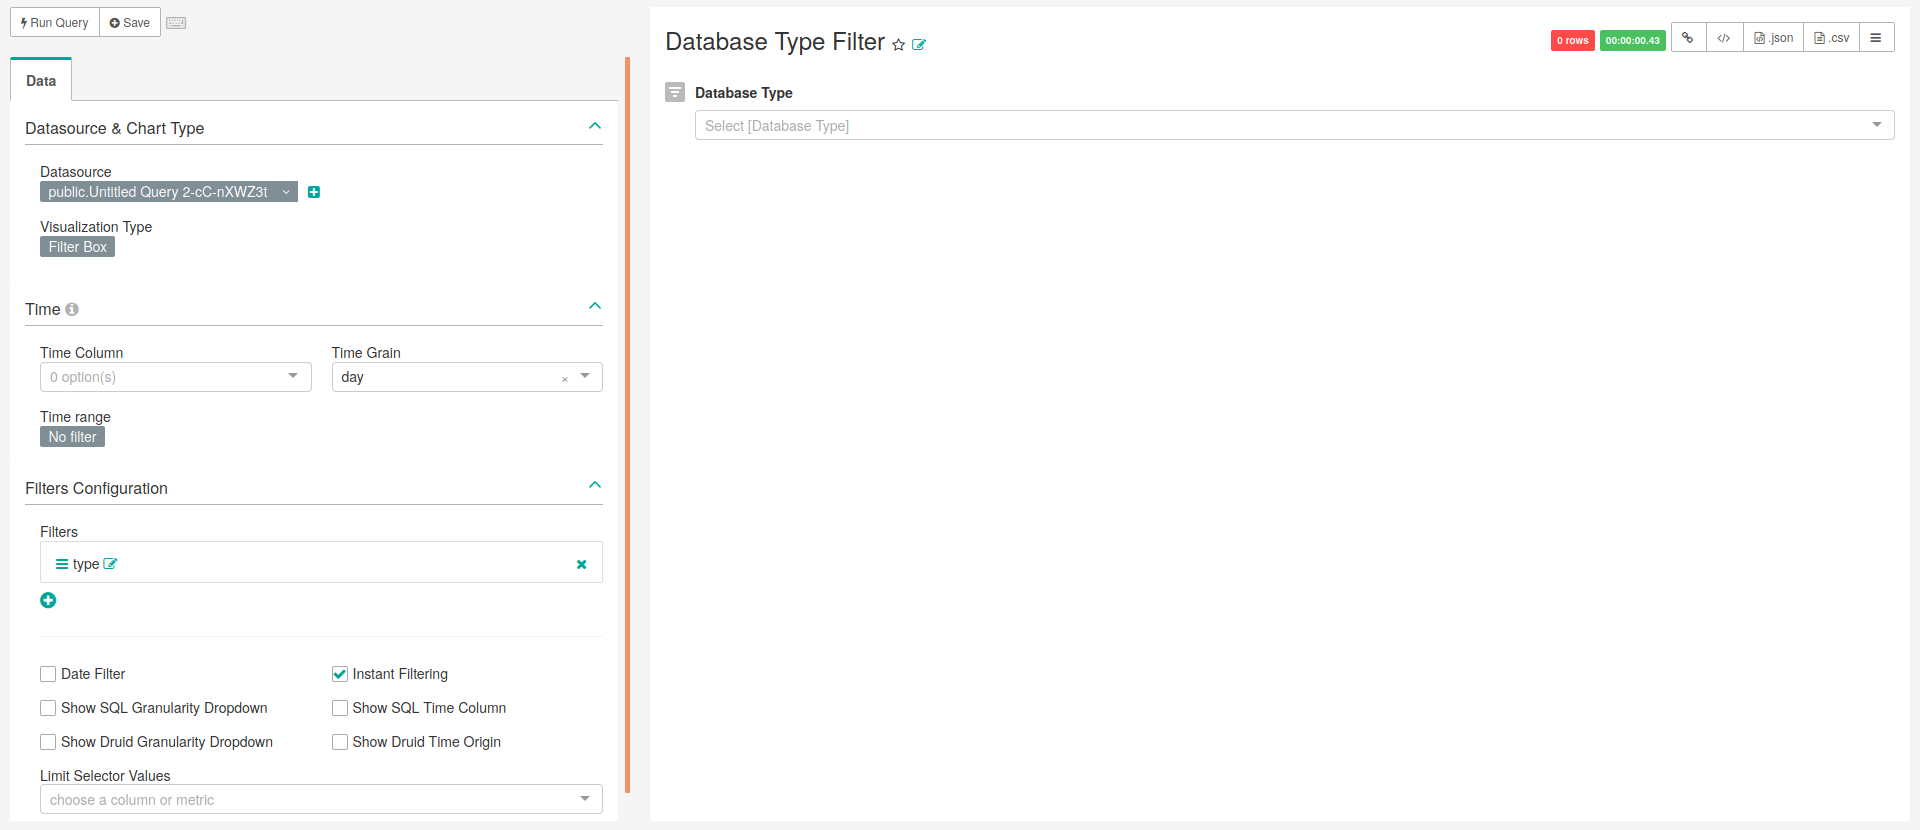
\includegraphics[width=1\linewidth]{images/databaseTypeFilter} \caption{Superset chart creation: Settings for creating the database type filter.}\label{fig:databaseTypeFilter}
\end{figure}

\section{Country Filter}\label{country-filter}

Discuss what is important to see in this chart\ldots{} TO DO

\subsection{SQL query}\label{sql-query}

\begin{Shaded}
\begin{Highlighting}[]
\CommentTok{--  Country and database type filters}
\KeywordTok{SELECT}\NormalTok{ source.name, }
\NormalTok{       country.country }\KeywordTok{AS}\NormalTok{ Country, }
\NormalTok{       database_type }\KeywordTok{AS} \KeywordTok{Type}\NormalTok{,}
\NormalTok{       source.slug}
\KeywordTok{FROM}\NormalTok{ public.data_source }\KeywordTok{AS} \KeywordTok{source} \KeywordTok{INNER} \KeywordTok{JOIN}\NormalTok{ public.country }
  \KeywordTok{AS}\NormalTok{ country }\KeywordTok{ON}\NormalTok{ source.country_id=country.id;}
\end{Highlighting}
\end{Shaded}

\subsection{Chart settings}\label{chart-settings-1}

TO DO

\section{General - World Map}\label{general---world-map}

Discuss what is important to see in this chart\ldots{} TO DO

\subsection{SQL query}\label{sql-query-1}

\begin{Shaded}
\begin{Highlighting}[]
\CommentTok{--    General - World Map}
\KeywordTok{SELECT}\NormalTok{  name,}
\NormalTok{        slug,}
\NormalTok{        release_date,}
\NormalTok{        database_type }\KeywordTok{AS} \KeywordTok{Type}\NormalTok{,}
\NormalTok{        latitude,}
\NormalTok{        longitude,}
        \KeywordTok{link}\NormalTok{,}
\NormalTok{        country }\KeywordTok{AS}\NormalTok{ Country,}
\NormalTok{        continent}
\KeywordTok{FROM}\NormalTok{ public.data_source }\KeywordTok{AS} \KeywordTok{source} \KeywordTok{INNER} \KeywordTok{JOIN}\NormalTok{ public.country }
  \KeywordTok{AS}\NormalTok{ country }\KeywordTok{ON}\NormalTok{ source.country_id=country.id;}
\end{Highlighting}
\end{Shaded}

\subsection{Chart settings}\label{chart-settings-2}

TO DO

\section{General - Network Growth
(Summary)}\label{general---network-growth-summary}

Discuss what is important to see in this chart\ldots{} TO DO

\subsection{SQL query}\label{sql-query-2}

\begin{Shaded}
\begin{Highlighting}[]
\CommentTok{-- 108    General - Network Growth (Summary)}
\KeywordTok{SELECT}\NormalTok{ data.source,}
\NormalTok{       data.country }\KeywordTok{AS}\NormalTok{ Country,}
\NormalTok{       data.database_type }\KeywordTok{AS} \KeywordTok{Type}\NormalTok{,}
       \CommentTok{--cast(stratum_1 as INTEGER )*30 AS Days,}
\NormalTok{       data.release_date - }\FunctionTok{cast}\NormalTok{(stratum_1 }\KeywordTok{AS} \DataTypeTok{INTEGER}\NormalTok{) * }\DataTypeTok{INTERVAL} 
        \StringTok{'1 month'} \KeywordTok{as} \DataTypeTok{Time}\NormalTok{,}
\NormalTok{       count_value                   }\KeywordTok{AS} \FunctionTok{count}
\KeywordTok{FROM}\NormalTok{ (}
     \KeywordTok{SELECT}\NormalTok{ source.name              }\KeywordTok{AS} \KeywordTok{source}\NormalTok{,}
\NormalTok{            achilles.analysis_id     }\KeywordTok{AS}\NormalTok{ analysis_id,}
\NormalTok{            achilles.stratum_1,}
\NormalTok{            achilles.stratum_2,}
\NormalTok{            achilles.stratum_3,}
\NormalTok{            achilles.stratum_4,}
\NormalTok{            achilles.stratum_5,}
\NormalTok{            achilles.count_value,}
\NormalTok{            country.country,}
\NormalTok{            source.database_type, }
\NormalTok{            source.release_date}
     \KeywordTok{FROM}\NormalTok{ public.achilles_results }\KeywordTok{AS}\NormalTok{ achilles }\KeywordTok{INNER} \KeywordTok{JOIN} 
\NormalTok{      public.data_source }\KeywordTok{AS} \KeywordTok{source} \KeywordTok{ON}
\NormalTok{      achilles.data_source_id=source.id}
     \KeywordTok{INNER} \KeywordTok{JOIN}\NormalTok{ public.country }\KeywordTok{AS}\NormalTok{ country }\KeywordTok{ON} 
\NormalTok{      source.country_id=country.id}
\NormalTok{     ) }\KeywordTok{data}
\KeywordTok{WHERE}\NormalTok{ analysis_id = }\DecValTok{108}\NormalTok{;}
\end{Highlighting}
\end{Shaded}

\subsection{Chart settings}\label{chart-settings-3}

TO DO

\section{General - Network Growth by
Date}\label{general---network-growth-by-date}

Discuss what is important to see in this chart\ldots{} TO DO

\subsection{SQL query}\label{sql-query-3}

\begin{Shaded}
\begin{Highlighting}[]
\CommentTok{-- 108    General - Network Growth by Date}
\KeywordTok{SELECT}\NormalTok{ data.source,}
\NormalTok{       data.country,}
\NormalTok{       data.database_type,}
       \FunctionTok{cast}\NormalTok{(stratum_1 }\KeywordTok{as} \DataTypeTok{Integer}\NormalTok{)*}\DecValTok{30} \KeywordTok{AS} \DataTypeTok{DAY}\NormalTok{,}
\NormalTok{       count_value                   }\KeywordTok{AS} \FunctionTok{count}
\KeywordTok{FROM}\NormalTok{ (}
     \KeywordTok{SELECT}\NormalTok{ source.name              }\KeywordTok{AS} \KeywordTok{source}\NormalTok{,}
\NormalTok{            achilles.analysis_id     }\KeywordTok{AS}\NormalTok{ analysis_id,}
\NormalTok{            achilles.stratum_1,}
\NormalTok{            achilles.stratum_2,}
\NormalTok{            achilles.stratum_3,}
\NormalTok{            achilles.stratum_4,}
\NormalTok{            achilles.stratum_5,}
\NormalTok{            achilles.count_value,}
\NormalTok{            country.country,}
\NormalTok{            source.database_type}
     \KeywordTok{FROM}\NormalTok{ public.achilles_results }\KeywordTok{AS}\NormalTok{ achilles }\KeywordTok{INNER} \KeywordTok{JOIN} 
\NormalTok{      public.data_source }\KeywordTok{AS} \KeywordTok{source} \KeywordTok{ON} 
\NormalTok{      achilles.data_source_id=source.id}
     \KeywordTok{INNER} \KeywordTok{JOIN}\NormalTok{ public.country }\KeywordTok{AS}\NormalTok{ country }\KeywordTok{ON} 
\NormalTok{      source.country_id=country.id}
\NormalTok{     ) }\KeywordTok{data}
\KeywordTok{WHERE}\NormalTok{ analysis_id = }\DecValTok{108}\NormalTok{;}
\end{Highlighting}
\end{Shaded}

\subsection{Chart settings}\label{chart-settings-4}

TO DO

\section{General - Patients per
Country}\label{general---patients-per-country}

Discuss what is important to see in this chart\ldots{} TO DO

\subsection{SQL query}\label{sql-query-4}

\begin{Shaded}
\begin{Highlighting}[]
\CommentTok{-- 1    General - Patients per Country}
\KeywordTok{SELECT}\NormalTok{ source.name,}
\NormalTok{       country.country,}
\NormalTok{       source.database_type,}
\NormalTok{       count_value }\KeywordTok{as}\NormalTok{ patient_count,}
\NormalTok{       source.slug}
\KeywordTok{FROM}\NormalTok{ public.achilles_results }\KeywordTok{AS}\NormalTok{ achilles }\KeywordTok{INNER} \KeywordTok{JOIN} 
\NormalTok{  public.data_source }\KeywordTok{AS} \KeywordTok{source} \KeywordTok{ON}\NormalTok{ achilles.data_source_id=source.id}
  \KeywordTok{INNER} \KeywordTok{JOIN}\NormalTok{ public.country }\KeywordTok{AS}\NormalTok{ country }\KeywordTok{ON} 
\NormalTok{  source.country_id=country.id}
\KeywordTok{WHERE}\NormalTok{ analysis_id = }\DecValTok{1}\NormalTok{;}
\end{Highlighting}
\end{Shaded}

\subsection{Chart settings}\label{chart-settings-5}

TO DO

\section{General - Database Types per
Country}\label{general---database-types-per-country}

Discuss what is important to see in this chart\ldots{} TO DO

\subsection{SQL query}\label{sql-query-5}

\begin{Shaded}
\begin{Highlighting}[]
\CommentTok{-- 1    General - Database types per Country}
\KeywordTok{SELECT}\NormalTok{ source.name, }
\NormalTok{       country.country }\KeywordTok{as}\NormalTok{ Country, }
\NormalTok{       database_type }\KeywordTok{as} \KeywordTok{Type}\NormalTok{,}
\NormalTok{       count_value }\KeywordTok{as} \OtherTok{"Nr_patients"}\NormalTok{,}
\NormalTok{       source.slug}
\KeywordTok{FROM}\NormalTok{ public.achilles_results }\KeywordTok{AS}\NormalTok{ achilles }\KeywordTok{INNER} \KeywordTok{JOIN} 
\NormalTok{  public.data_source }\KeywordTok{AS} \KeywordTok{source} \KeywordTok{ON}\NormalTok{ achilles.data_source_id=source.id}
  \KeywordTok{INNER} \KeywordTok{JOIN}\NormalTok{ public.country }\KeywordTok{AS}\NormalTok{ country }\KeywordTok{ON} 
\NormalTok{  source.country_id=country.id}
\KeywordTok{WHERE}\NormalTok{ analysis_id = }\DecValTok{1}\NormalTok{;}
\end{Highlighting}
\end{Shaded}

\subsection{Chart settings}\label{chart-settings-6}

TO DO

\chapter{Person}\label{person}

\chapter{Population Characteristics}\label{population-characteristics}

\chapter{Visit}\label{visit}

\chapter{Death}\label{death}

\chapter{Concepts}\label{concepts}

\chapter{Data Domains}\label{data-domains}

\bibliography{refs.bib}

\end{document}
